\documentclass[10pt, a4paper]{article}

\usepackage[utf8]{inputenc}
\usepackage[english]{babel}
\usepackage[english]{isodate}
\usepackage[parfill]{parskip}
\usepackage{graphicx}
\usepackage[utf8]{inputenc}
\usepackage[section]{placeins}
\usepackage{float}
\usepackage{listings}
\usepackage{color}

\definecolor{dkgreen}{rgb}{0,0.6,0}
\definecolor{gray}{rgb}{0.5,0.5,0.5}
\definecolor{mauve}{rgb}{0.58,0,0.82}

\lstset{
  frame=tb,
  language=C++,
  aboveskip=3mm,
  belowskip=3mm,
  showstringspaces=false,
  columns=flexible,
  basicstyle={\small\ttfamily},
  numbers=none,
  numberstyle=\tiny\color{gray},
  keywordstyle=\color{blue},
  commentstyle=\color{dkgreen},
  stringstyle=\color{mauve},
  breaklines=true,
  breakatwhitespace=true,
  tabsize=3
}

\author{Elwin Cabrera}
\title{Alternating-Bit, Go-Back-N, and Selective Repeat Analysis}

\begin{document}

\pagenumbering{Roman}

\maketitle
\newpage

\tableofcontents
\newpage

\listoffigures
\newpage

\pagenumbering{arabic}

\section{Academic Integrity}
    I have read and understood the course academic integrity policy.
\section{Protocol Implementations}
    
  \subsection{Alternating-Bit}
    \subsubsection{A Output\label{abt-aout}}
        The first thing that this function does is wait on some data from layer 5 to be sent to B. The program then encapsulates
this data into a packet that we can send to layer 3 later. Once the data is in a packet its then put into a queue and if no packets are currently in the link or if the program is not trying to resolve a corrupt packet then we pop that packet from the queue, set our current packet to the packet we just popped, and send it down to layer 3 and start a timer. However, if a packet is currently using the link or if the program is trying to resolve a corrupt packet (can occur under high corruption thus will take long for B to receive a valid packet ) then we just keep that packet in the queue for later transmission.  
    \subsubsection{A Input\label{abt-ain}}
        A only gets acknowledgment packets from B so that is the only type of packets that A Input handles. When A Input gets a packet it first checks if that packet is valid and not corrupt. After the validation, it then checks if the acknowledgment number corresponds to the latest packet that A sent. If the acknowledgment number is equal to the last packet A sent, then A will stop the timer and check if the queue has any more packets to transmit if yes then it will pop from the queue, start a timer,  and then send next packet to layer 3.  
    \subsubsection{A Interrupt\label{abt-aint}}
        The interrupt mechanism used for this protocol is simple. Every time that A sends a new packet it starts a timer. The only time that the timer is stopped is when A receives an acknowledgment for the current packet and when the A Interrupt function is called. When A Interrupt is called it simply re-transmits the current packet that is saved as a variable as ``struct pkt current\_pkt''.
    \subsubsection{B Input\label{abt-bin}}
        When B first gets a packet it checks if the packet is valid and not corrupt and then checks if the packet is a duplicate. If the packet is a duplicate it simply sends an acknowledgment corresponding to that duplicate packet. If the packet if not valid then B will just return. However, if the packet is valid and if it's not a duplicate packet then it sends the data to the application and then sends an acknowledgment packet corresponding the packet B just received. 

  \subsection{Go-back-N}
    \subsubsection{A Output\label{gbn-aout}}
        This function is similar to the alternating bit's version of A Output in \ref{abt-aout}, with only two modifications. The first modification is the introduction of a window of packets which is just an array of packets of size N where N is the window size which is specified by the user running the program. The second modification is that instead of having only one packet in the link we can send as many packets to layer 3 as long as the window is not full, if the window is full then we just push that packet in a queue. 
    \subsubsection{A Input\label{gbn-ain}}
        This function does something similar to the alternating bit version of A Input in \ref{abt-ain} with only one change. Since we introduced the window we have to check the acknowledgment against the first packet in our window, this is because our window can't move unless the first packet in the window is acknowledged. When the first packet in our window is acknowledged then we shift our window right up until the next unacknowledged packet and then we push more packets into the window if our queue of buffered packets is not empty. An interesting thing that this function does is that if the acknowledgment does not correspond to the first packet in the window then it does nothing this is explained in in the next section \ref{gbn-aint}. 
    \subsubsection{A Interrupt\label{gbn-aint}}
        The interrupt mechanism is simple. Whenever a new packet is the first packet in the window then a timer is started. When that timer runs out, which means that the first packet in the window was not acknowledged in time, then A sends all packets that are currently in that window to layer 3. This means that whenever A gets an acknowledgment packet it doesn't care if the acknowledgment packet is not the expected acknowledgment in which case A will just wait for the timer to run out to re-transmit the window. This can be problematic under high loss or high corruption rate as the program will keep sending the entire window often causing long execution time.
    \subsubsection{B Input\label{gbn-bin}}
        Here it just checks if the packet is valid, if not then it just finishes and does not send an acknowledgment. Then it checks if the packet just received is a duplicate if it's not then it sends the data to the application. Finally regardless if the packet is a duplicate or not it sends an acknowledgment corresponding to the packet just received.

  \subsection{Selective Repeat}
    \subsubsection{A Output\label{sr-aout}}
        The implementation for this function is nearly identical to Go-Back-N's version of A Output  see section \ref{gbn-aout}. The only difference is that a packet is encapsulated in a different structure called ``struct pkt\_info'' and that is what gets pushed to the queue, the struct used is shown below.
        
        \begin{lstlisting}
            struct pkt_info{
                bool pkt_acked;
                bool app_deliverd;
                int timeout;        // <- this is the important part
                struct pkt pkt;
            };
        \end{lstlisting}

        After we put a packet in this structure we set a timeout for that packet by adding the current time and the time interval we want that packet to timeout in the future.
    \subsubsection{A Input}
        This function behaves in the same way that Go-Back-N's A Input does in section \ref{gbn-ain}
    \subsubsection{A Interrupt\label{sr-aint}}
        The interrupt implementation for this protocol is the most interesting out of all three protocols this is because each packet needs to have its own timer but we only have available one timer interrupt. To achieve this we need a way to implement multiple logical timers from one given timer. What I decided to do was to start the timer once in the beginning and have it interrupt very often endlessly. I decided to have the timer interrupt once every 1-time unit (I could have gone lower if I wanted to be more accurate). Since the timer is interrupting very often all I have to do is have an int or float variable that corresponds to each packet and every time an interrupt happens I check all packets and their timeouts to see if the time at this moment is equal to the packets timeout, if yes then I send that one packet to layer 3. This is why a packet is encapsulated in a different struct because we need to hold extra information about the packet.    
    \subsubsection{B Input\label{sr-bin}}
        In the previous protocols, B didn't change much. With selective repeat B now also has a window and its implemented in the same way that A's window is implemented. Another difference from the previous protocols is that whenever B gets a packet that is out of order then it buffers that packet by putting it in a queue so when its time for that packet to be sent to the application B already has it and can deliver it in order right away.
    
\section{Experiments}
    Two experiments were done to test how effective or ineffective each of the three protocols were. Through each experiment three variables were kept constant the total number of messages was 1000 to be sent by entity A, a mean time of 50 between message arrivals (from A’s layer5) and a corruption probability of 0.2. 
    
  \subsection{Average Throughput vs Loss Probability}
    This experiment tests the average throughput on different loss probabilities for protocols Alternating-Bit (\ref{exp1-abt}), Go-Back-N (\ref{exp1-gbn}), and Selective Repeat (\ref{exp1-sr}). The loss probabilities that were measured were 0.1, 0.2, 0.4, 0.6, and 0.8. There were two versions of this experiment done on protocols Go-Back-N (\ref{exp1-gbn}) and Selective Repeat (\ref{exp1-sr}) for window size of 10 and then window size of 50.  Below were the results. 
    
    \begin{figure}[H]
        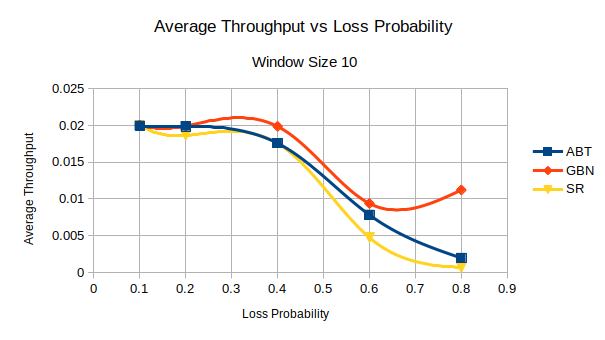
\includegraphics[width=\textwidth]{exp1-w10.png}
        \centering
        \caption{Avg. Throughput vs Loss Probability -  Window 10 }
        \label{fig:exp1-w10}
    \end{figure}
    
    \begin{figure}[H]
        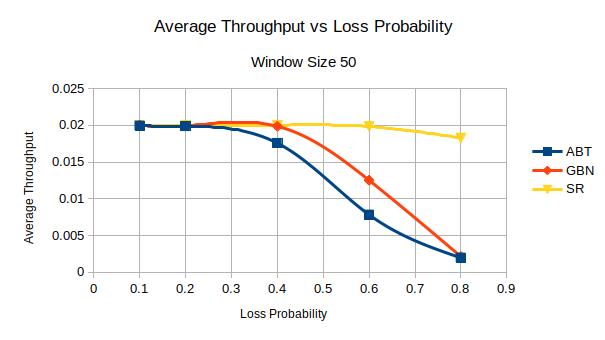
\includegraphics[width=\textwidth]{exp1-w50.png}
        \centering
        \caption{Avg. Throughput vs Loss Probability - Window 50 }
        \label{fig:exp1-w50}
    \end{figure}
    
    \subsubsection{Alternating-Bit\label{exp1-abt}}
      Before running this experiment I expected for the throughput to decrease when the loss probability was increased for this protocol. After running the experiments and seeing the results we see that the throughput stays relatively high until the loss probability is 0.4 or greater is when you see a significant change in throughput. Also since this protocol does not use window there is only one version of this experiment.
    
    \subsubsection{Go-back-N\label{exp1-gbn}}
        Before running this experiment I expected to see that this protocol would a do a little better than Alternating-Bit in section \ref{exp1-abt}. What we see based on the results shown above is that this protocol only does slightly better than Alternating-Bit, \ref{exp1-abt}. The protocol stays at a higher throughput just a little longer past 0.4 loss probability then the throughput starts to decline at the same rate as in Alternating-Bit. In the first version, where we use window of size 10, we see that there's an increase in throughput right after 0.7 loss probability. This could be due to many factors such as my implementation, randomized sequence packets were bring lost, or even bad code.   
      
    \subsubsection{Selective Repeat\label{exp1-sr}}
    
        The results for this experiment were very interesting ant not what I predicted before looking at the data. What my thoughts were before I ran this experiment was tat Selective Repeat would do better than all protocols tested previously. The results of this experiment were interesting and not what I was expecting. In the first version with window size of 10 shown in figure \ref{fig:exp1-w10}, the data shows that Selective Repeat did worse than all the last two protocols in the previous sections. This was surprising considering that Selective Repeat had extra functionalities that would help with throughput that the other two protocols didn't. However, a look figure \ref{fig:exp1-w50} showed that this protocol indeed did better than the previous ones as it stayed at high throughput for much longer and declined slowly as the loss probability went up. A possible explanation in such a big difference between the two version could be that Selective Repeat does not do well when the window size is low, I con
    
  \subsection{Average Throughput vs Window Size}
    This experiment tests the average throughput on different window sizes for protocols Alternating-Bit (\ref{exp1-abt}), Go-Back-N (\ref{exp1-gbn}), and Selective Repeat (\ref{exp1-sr}). The window sizes that were measured were 10, 50, 100, 200, and 500. There were 3 versions of this experiment each with different loss probabilities done on all three protocols they were loss of 0.2, 0.5, and 0.8. Below were the Results of all the three protocols with different loss probability conditions. 
    
    \begin{figure}[H]
        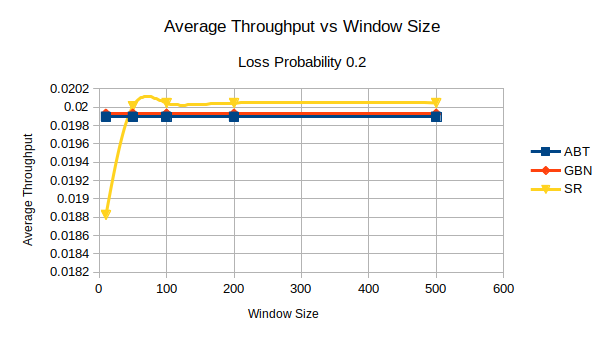
\includegraphics[width=\textwidth]{exp2-l02.png}
        \centering
        \caption{Avg. Throughput vs Window Size - Loss 0.2 }
        \label{fig:exp2-l0.2}
    \end{figure}
      
    \begin{figure}[H]
        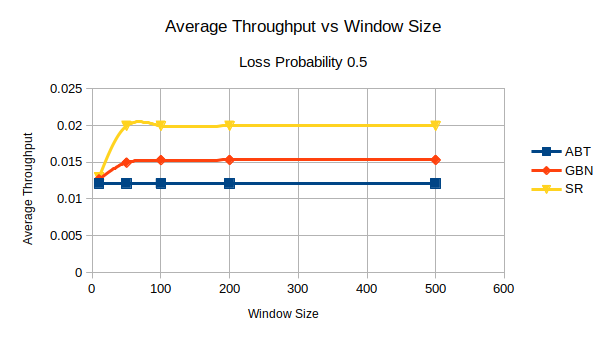
\includegraphics[width=\textwidth]{exp2-l05.png}
        \centering
        \caption{Avg. Throughput vs Window Size - Loss 0.5  }
        \label{fig:exp2-l0.5}
    \end{figure}
        
    \begin{figure}[H]
        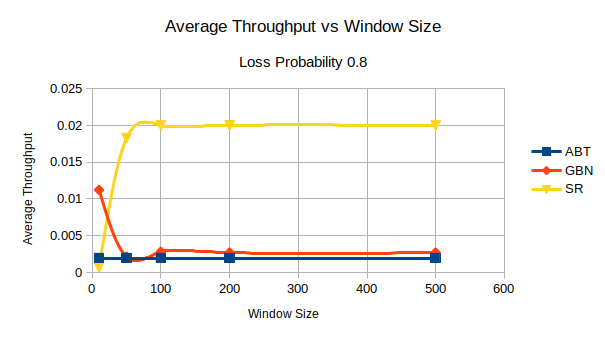
\includegraphics[width=\textwidth]{exp2-l08.png}
        \centering
        \caption{Avg. Throughput vs Window Size - Loss 0.8 }
        \label{fig:exp2-l0.8}
    \end{figure}
    
    \subsubsection{Alternating-Bit}
    
    
        Since this protocol does not depend on the window size it was expected that for each condition that the throughput would remain constant. The data in figures \ref{fig:exp2-l0.2}, \ref{fig:exp2-l0.5}, and \ref{fig:exp2-l0.8} indeed that this protocol stayed constant when the window size changed with only slight variations in throughput when the loss probability changed. 
        
      
    \subsubsection{Go-back-N}
    
        According to the data figures \ref{fig:exp2-l0.2}, \ref{fig:exp2-l0.5}, and \ref{fig:exp2-l0.8} this protocol only does well when the window size and loss probabilities are small. When the window size gets too big and the loss probability increases the throughput approaches zero. This is due to the fact that when the timer expires for the first packet in the window then the entire window is sent, this can be problematic when you have a big window and a high loss probability.  
        
        
    \subsubsection{Selective Repeat}
    
        As always selective repeat gives is interesting results. We can see from the data that selective repeat does better than the other two protocols the majority of the time. The reason why the results from this experiments were interesting were because surprisingly this protocol did worse than the other two when the window size was small (less than 50) but better when it was large (grater than 50). This confirms my earlier inference in section \ref{exp1-sr} from the first experiment.
    
       

  \subsection{Packets Received by Application vs Loss Probability \label{exp3}}
	
	This experiment tests the average number of packets received at B by the application on different loss probabilities for protocols Alternating-Bit (\ref{exp1-abt}), Go-Back-N (\ref{exp1-gbn}), and Selective Repeat (\ref{exp1-sr}). The loss probabilities that were measured were 0.1, 0.2, 0.4, 0.6, and 0.8. There were two versions of this experiment done on protocols Go-Back-N (\ref{exp1-gbn}) and Selective Repeat (\ref{exp1-sr}) for window size of 10 and then window size of 50.  Below were the results.
	
	\begin{figure}[H]
        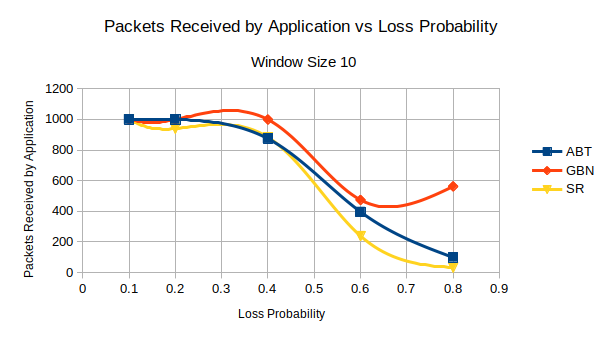
\includegraphics[width=\textwidth]{exp3-w10.png}
        \centering
        \caption{Avg. Packets Received by Application vs Loss Prob. -  Window 10 }
        \label{fig:exp3-w10}
    \end{figure}
    
    \begin{figure}[H]
        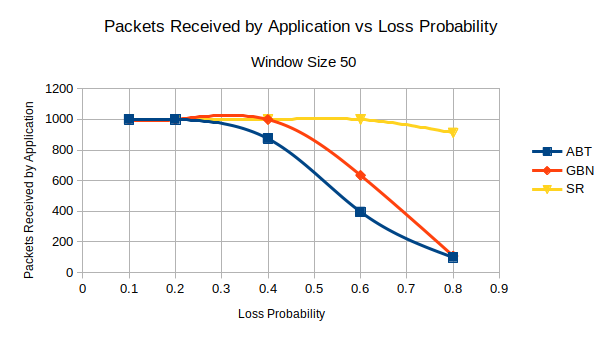
\includegraphics[width=\textwidth]{exp3-w50.png}
        \centering
        \caption{Avg. Packets Received by Application vs Loss Prob. - Window 50 }
        \label{fig:exp3-w50}
    \end{figure}
	
    \subsubsection{Alternating-Bit}
    	
    	In the graphs above you can see that this protocol did the same in both version, which is what is expected since this protocol does not depend on the window size and the data reflects that. In the first version of this experiment the rate of packets received at application declined slower than that of Selective Repeat protocol, which is interesting as Selective Repeat utilizes the link more. Around loss probability 0.4 is where this protocol starts to loose packets at the application at a faster rate.
    
    \subsubsection{Go-back-N}
	    
	    Similar to Alternating-Bit this protocol starts to loose packets at the application at B faster rate after loss probability of 0.4 on both versions. In figure \ref{fig:exp3-w10} this protocol did better than the other two in that the rate decline of packets received at the application was the slowest. In figure \ref{fig:exp3-w50} the decline rate was slower than in the figure \ref{fig:exp3-w10} but this time it was not the slowest.
	    
    \subsubsection{Selective Repeat}
    	
    	This protocol gave the most interesting results in that the results from each figure was drastically different. in figure \ref{fig:exp3-w10} this protocol this the worst compared to the other two protocols. However, when the window was increased form 10 to 50 as shown in figure \ref{fig:exp3-w50} showed significant improvements. In figure \ref{fig:exp3-w50} the number of packets that the application got at B was closer to 100\% most of the time.   
    
  \subsection{Packets Received by Application vs Window Size \label{exp4}}
  
     This experiment tests the average number of packets received at B by the application on different window sizes for protocols Alternating-Bit (\ref{exp1-abt}), Go-Back-N (\ref{exp1-gbn}), and Selective Repeat (\ref{exp1-sr}). The window sizes that were measured were 10, 50, 100, 200, and 500. There were 3 versions of this experiment each with different loss probabilities done on all three protocols they were loss of 0.2, 0.5, and 0.8. Below were the Results of all the three protocols with different loss probability conditions. 
     
    \begin{figure}[H]
        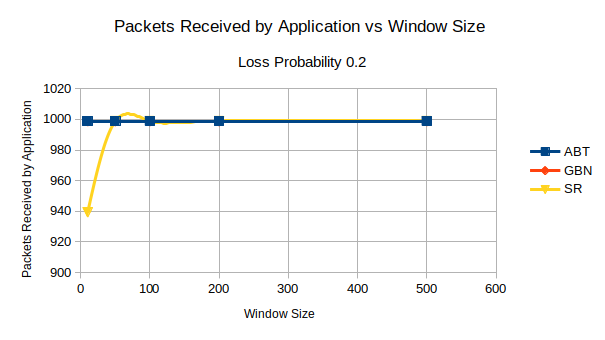
\includegraphics[width=\textwidth]{exp4-l02.png}
        \centering
        \caption{Avg. Packets Received by Application vs Window Size - Loss 0.2 }
        \label{fig:exp4-l0.2}
    \end{figure}
      
    \begin{figure}[H]
        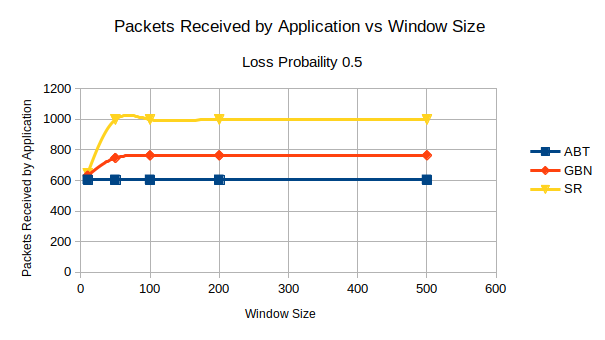
\includegraphics[width=\textwidth]{exp4-l05.png}
        \centering
        \caption{Avg. Packets Received by Application vs Window Size - Loss 0.5  }
        \label{fig:exp4-l0.5}
    \end{figure}
        
    \begin{figure}[H]
        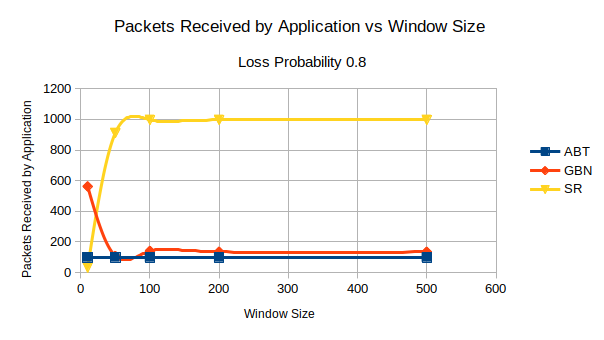
\includegraphics[width=\textwidth]{exp4-l08.png}
        \centering
        \caption{Avg. Packets Received by Application vs Window Size - Loss 0.8 }
        \label{fig:exp4-l0.8}
    \end{figure}
     
    \subsubsection{Alternating-Bit}
    
	    As mentioned before the window size is does not impact this protocol so I expected for the packets received at the application to stay constant when the window is increased. Figures \ref{fig:exp4-l0.2}, \ref{fig:exp4-l0.5}, \ref{fig:exp4-l0.8} show exactly what we already knew about the relationship with the window size and this protocol. The figures above also show that this protocol never did better than the other two protocols. Every time that the loss probability was increased the number of packets received at at the application decreased. 
	    
    \subsubsection{Go-back-N}
    
	    In figure \ref{fig:exp4-l0.2} that the application received 100\% of the packets with this protocol with increasing window. Its not until we start to increase the loss probability that this protocol starts to decline in the number of packets received by the application. In figure \ref{fig:exp4-l0.8} we see that the application received almost no packets and is about the same with Alternating-Bit.
	    
    \subsubsection{Selective Repeat}
    
    	from the figures above we see consistent results across the board for this protocol. The data shows us that this protocol does well only when the window size is large enough, more than 100 in this case. If the window size is too small and the loss probability is high then this protocol does worse than the other two we see this in figure \ref{fig:exp4-l0.8} when the window size is around 10 the number of packets that the application received was almost 0. 

  \subsection{Average Total Time vs Window Size\label{exp5}}
  
    This experiment tests the average total time it takes for each protocol to finish on different window sizes for protocols Alternating-Bit (\ref{exp1-abt}), Go-Back-N (\ref{exp1-gbn}), and Selective Repeat (\ref{exp1-sr}). The window sizes that were measured were 10, 50, 100, 200, and 500. There were 3 versions of this experiment each with different loss probabilities done on all three protocols they were loss of 0.2, 0.5, and 0.8. Below were the Results of all the three protocols with different loss probability conditions. 
    
    \begin{figure}[H]
        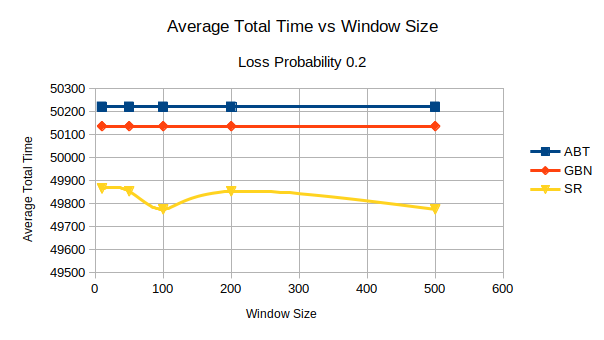
\includegraphics[width=\textwidth]{exp5-l02.png}
        \centering
        \caption{Avg. Total Time vs Window Size - Loss 0.2 }
        \label{fig:exp5-l0.2}
    \end{figure}
      
    \begin{figure}[H]
        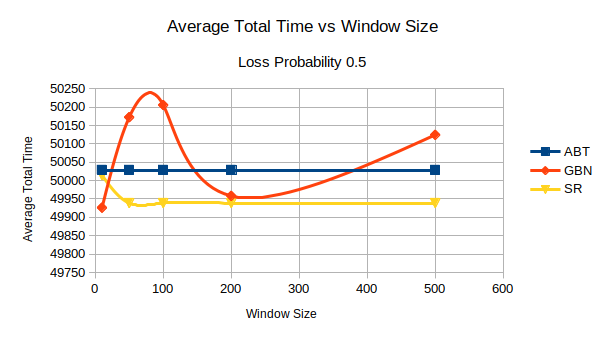
\includegraphics[width=\textwidth]{exp5-l05.png}
        \centering
        \caption{Avg. Total Time vs Window Size - Loss 0.5  }
        \label{fig:exp5-l0.5}
    \end{figure}
        
    \begin{figure}[H]
        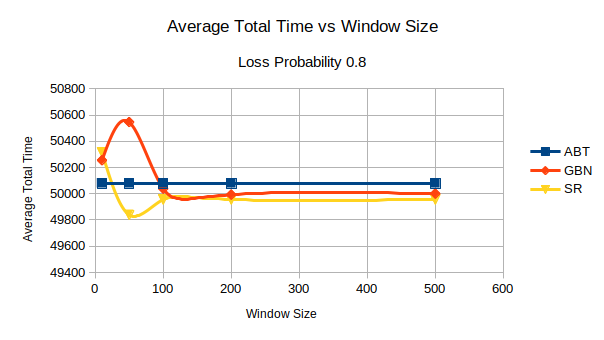
\includegraphics[width=\textwidth]{exp5-l08.png}
        \centering
        \caption{Avg. Total Time vs Window Size - Loss 0.8 }
        \label{fig:exp5-l0.8}
    \end{figure}
    
    \subsubsection{Alternating-Bit}
        
        Again since this protocol does not depend on window size we expect to see that as the window size increases that the average total time stays the same for each version of this experiment, and that's exactly what each figure above shows. What was interesting here is that in figure \ref{fig:exp5-l0.2} with loss probability 0.2 we see that the time was the highest, but in figure \ref{fig:exp5-l0.5} with loss probability of 0.5 the average time is actually lower than that of the lower loss probability. This could be because the program terminates before it got to transmit all of the packets. Lastly figure \ref{fig:exp5-l0.8} we see the same results than that of figure \ref{fig:exp5-l0.8}.
    
    \subsubsection{Go-back-N}
        
        In figure \ref{fig:exp5-l0.5} shows some that time went down when window size was increased from 100 to 200 and then back up when increased some more. This could be a mistake in implementation or just that the simulator terminates early. In figure \ref{fig:exp5-l0.2} we see some impressive and interesting results as we increased the window size the time stayed constant. Lastly in figure \ref{fig:exp5-l0.8} we see that the average time was lower than that in figure \ref{fig:exp5-l0.2} which again could be due to the fact that the simulator terminates early.
    
    \subsubsection{Selective Repeat}
        
        This protocol had the lowest average time compared to the other two on all versions of this experiment. Also the average time did not change much with varying loss probabilities or window size , it was constant most of the time.

\end{document}
